\documentclass[12pt]{article}
\usepackage{amsmath}
\usepackage{graphicx}
\title{Report for Auto Control Lab11}
\date{2020/11/24}
\author{Jacky Yeh 4107064003}

\begin{document}
\begin{titlepage}

\maketitle
\end{titlepage}


\section{Introduction}
This is the eleventh Experiment of Auto Control Lab where TAs taught us the plot of root locus and the finding for the determination of the stability.


\section{LAB11}
\subsection{Part 1 Homework problems and its codes}
Objective:To perform operations to find out the ROOT LOCUS located at the LHP, also find out the minimum value of k!\\

These are the stated Homework problems\\

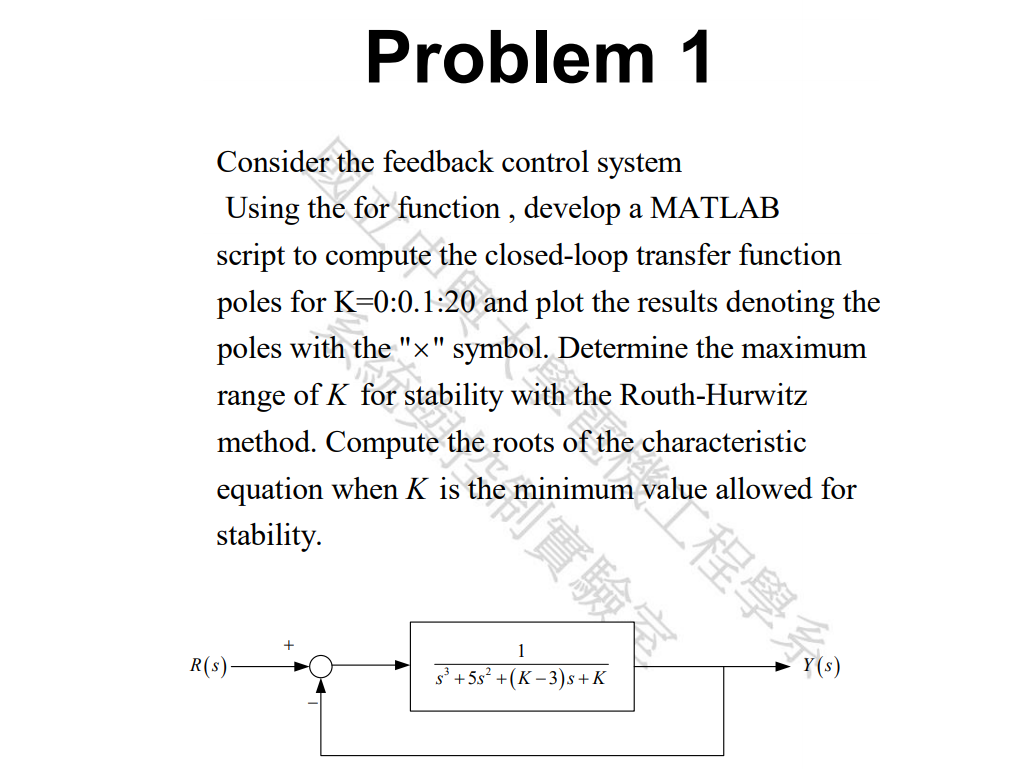
\includegraphics[scale=0.6]{Problem1.png} \\

\cleardoublepage
\subsection{CODES FOR PROBLEM1}
In order to perform the tasks, Matlab codes are needed. The following is the code needed for plotting\\
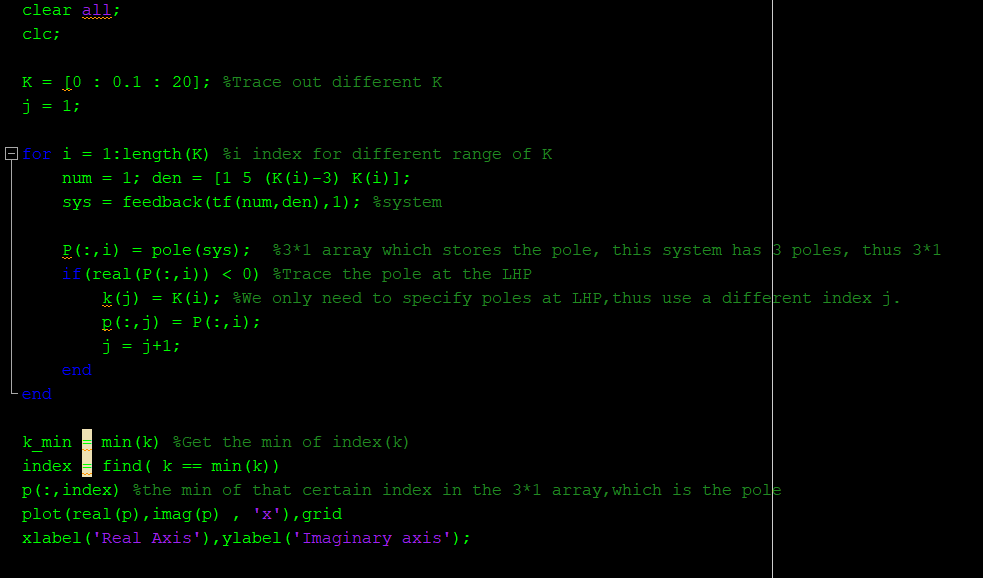
\includegraphics[scale=0.6]{Code1.png} \\

\subsection{Result of the Code and the plot of the ROOT LOCUS also the minimum k value}
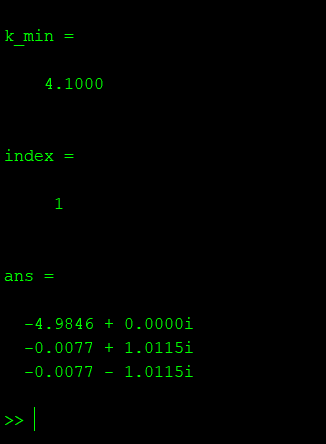
\includegraphics[scale=0.7]{Result1.png}\\
\cleardoublepage
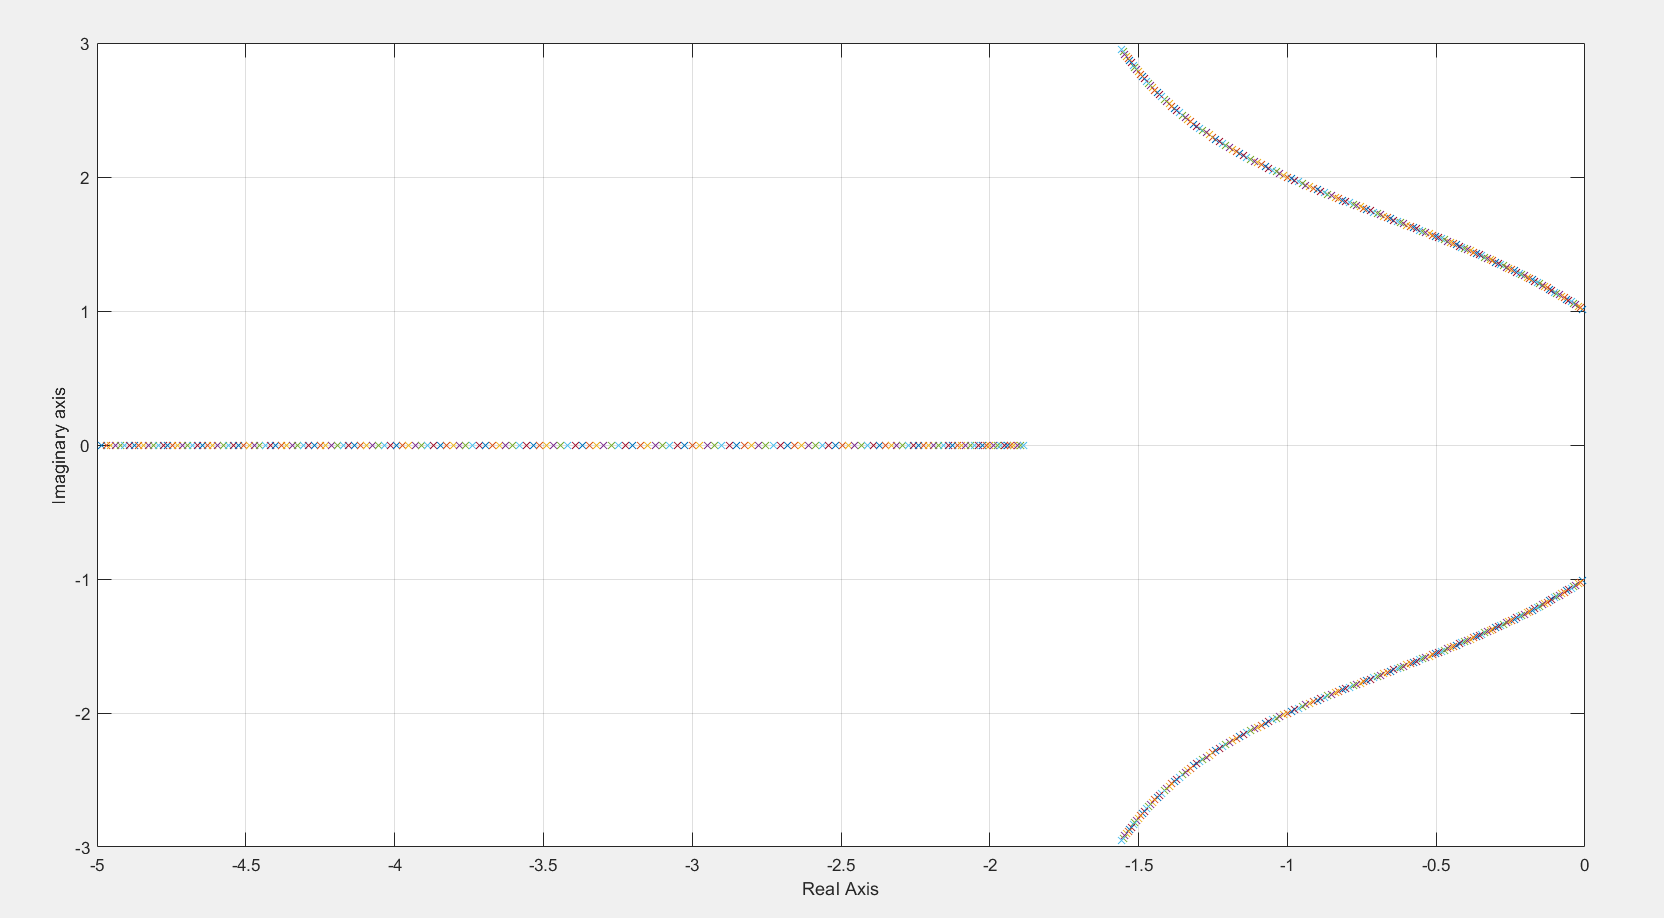
\includegraphics[scale=0.5]{Plot1.png}\\

\cleardoublepage


\subsection{Part 2 Homework problems}
Objective:To plug in and plot out the ROOT LOCUS FOR THE SPECIFIED feedback system located at LHP.

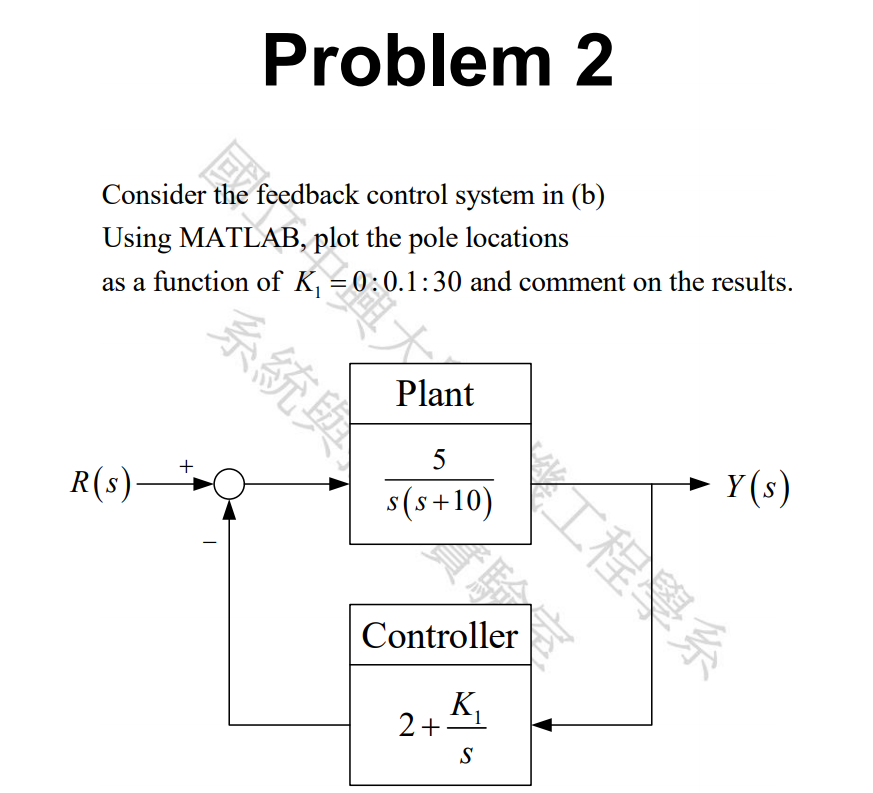
\includegraphics[scale=0.8]{Problem2.png}   \\

\cleardoublepage
\subsection{CODE FOR Part2}
In order to perform the tasks, Matlab codes are needed. The following code is used for plotting the system with different damping ratios and natural frequency \\

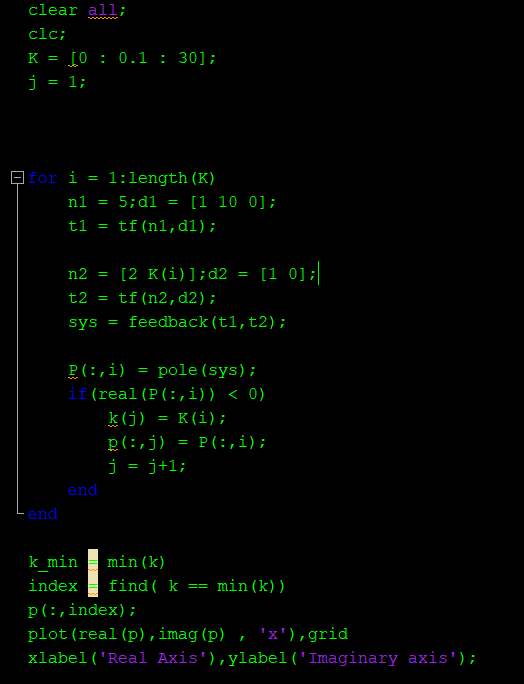
\includegraphics[scale=0.8]{Code2.png} \\

\cleardoublepage


\subsection{Plot out the root locus for the given feedback system!}
The following is the ROOT LOCUS of the system\\

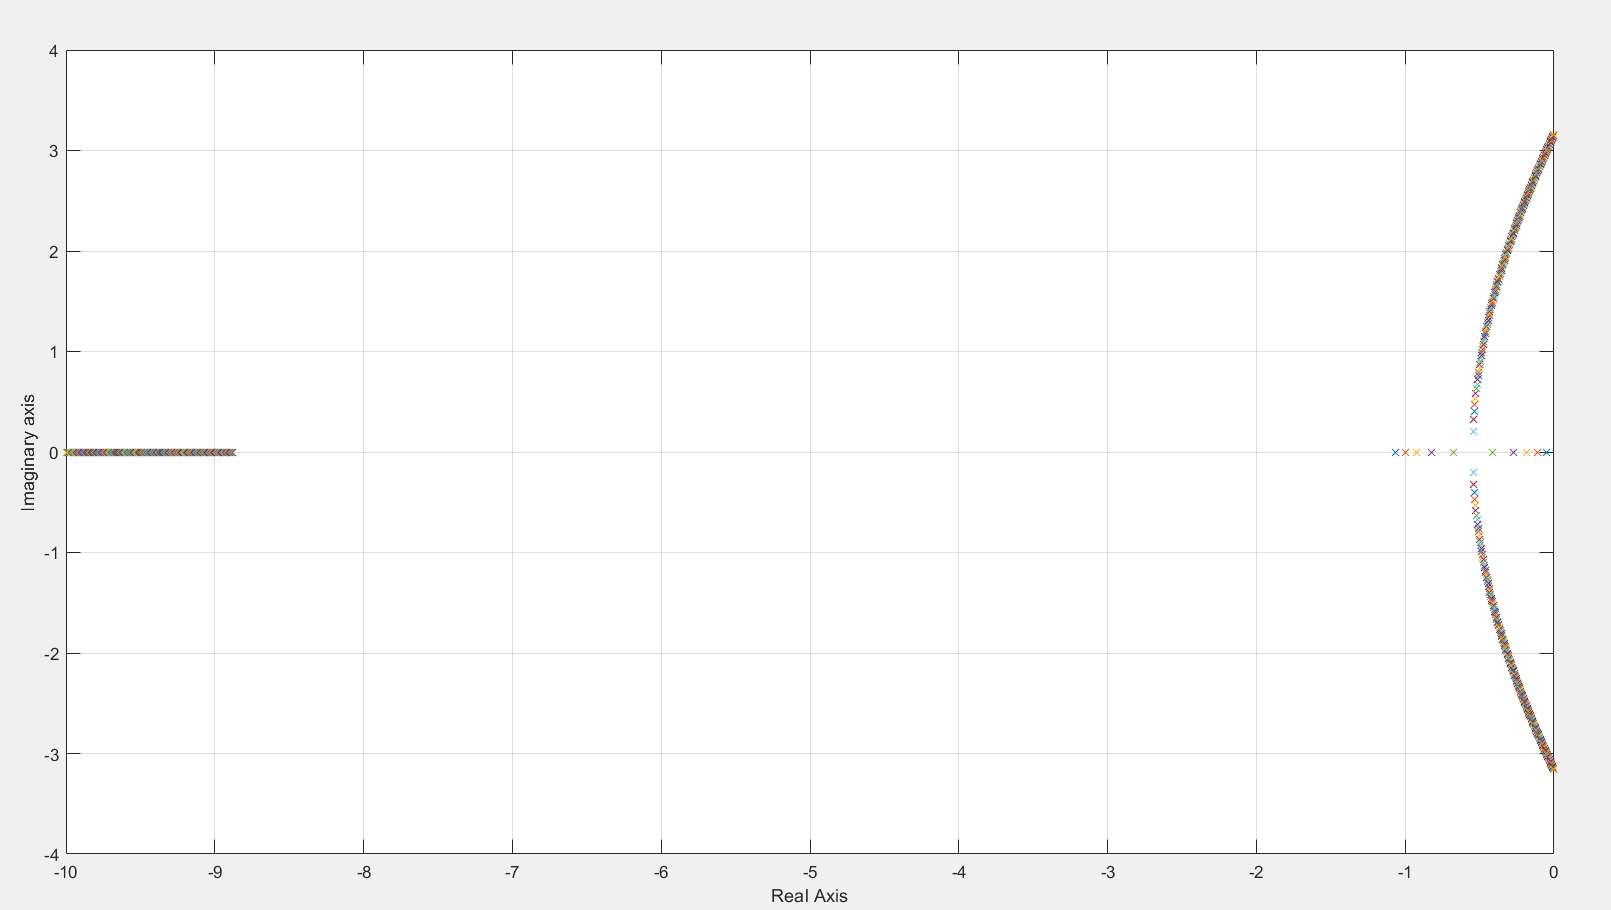
\includegraphics[scale=0.4]{Result2.png}\\


\section{Conclusion}
Today we learn how to plot the root locus of the system which is related to what we are learning right now, i.e the root locus plotting. Although originally, root locus plotting involves lots of trivial steps, including finding centroids of the poles, finding angle for asymptotes, also the intersections of imaginary axis with the root locus. By using MATLAB, these trivial stuff can be simplified, thus proved that MATLAB is a powerful tool for system analysis!

\begin{center}
This concludes the eleventh Week of Auto Control LAB\\
\end{center}

\end{document}
